\documentclass[11pt]{amsart}
\usepackage{amsmath,amsthm, amscd, amssymb, amsfonts, mathtools,color}
%\usepackage{tabu}
\usepackage[all]{xy}
\usepackage{mathrsfs}
\usepackage{enumitem}
\usepackage[T2A,T1]{fontenc}
%\usepackage{rotating}
\usepackage{multicol}
\newcommand{\pinom}{\genfrac{[}{]}{0pt}{}}
\usepackage{hyperref}

\allowdisplaybreaks

%\usepackage[basic,optics]{circ}
%\usepackage[spanish]{babel}
\usepackage[ansinew]{inputenc}
\usepackage{graphicx,fancyhdr}

%\usepackage[dvips, dvipsnames, usenames]{color}
\newcommand{\com}[1]{\textcolor{blue}{\textbf{#1}}}
\newcommand{\diag}{\operatorname{diag}}



\newcommand{\pre}{\mathfrak{Pre}}
\newcommand{\pref}{\mathfrak{Pre}_\textrm{fGK}}

\newcommand{\post}{\mathfrak{Post}}
\newcommand{\postf}{\mathfrak{Post}_{\textrm{fGK}}}

\newcommand{\deriv}{\mathfrak d}
\newcommand{\derv}{\mathfrak D}

\newcommand{\Lie}{\operatorname{Lie}}

\newcommand{\nucleo}{\mathbf R}
\newcommand{\Nuc}{\mathcal O}
\newcommand{\gen}{\mathbf{g}}
\newcommand{\Gb}{\mathbf G}
\newcommand{\Hb}{\mathbf H}
\newcommand{\Bb}{\mathbf B}
\newcommand{\uno}{{\mathbf 1}}

\newcommand{\ya}{\mbox{\usefont{T2A}{\rmdefault}{m}{n}\cyrya}}
\newcommand{\zh}{\bx}%{\mbox{\usefont{T2A}{\rmdefault}{m}{n}\cyrzh}}
\newcommand{\Zh}{\mathbb X}%{\mbox{\usefont{T2A}{\rmdefault}{m}{n}\CYRZH}}


\newcommand{\supp}{\operatorname{supp}}
\newcommand{\verma}{M}

\newcommand{\hopfuno}{\mathtt{H}}
\newcommand{\hopfdos}{\mathtt{K}}
\newcommand{\hopfdouble}{\mathtt{D}}
\newcommand{\xb}{x}%{\mathbf x}
\newcommand{\ub}{u}%{\mathbf u}


\numberwithin{equation}{section}
\newtheorem{theorem}{Theorem}[section]
\newtheorem{lemma}[theorem]{Lemma}
\newtheorem{coro}[theorem]{Corollary}
\newtheorem{conjecture}[theorem]{Conjecture}
\newtheorem{prop}[theorem]{Proposition}
\newtheorem{claim}{Claim}[section]

\newtheorem{paso}{Step}

\theoremstyle{definition}
\newtheorem{definition}[theorem]{Definition}
\newtheorem{example}[theorem]{Example}
\newtheorem{question}{Question}
\newtheorem{problem}{Problem}
\newtheorem*{strategy}{Strategy}
\newtheorem{notation}{Notation}


\newtheorem{xca}[theorem]{Exercise}
\theoremstyle{remark}
\newtheorem{remark}[theorem]{Remark}

\newtheorem{step}{Case}
\newtheorem{case}{Case}
\newtheorem{caso}{Step}
\newtheorem{posi}{}[caso]

\newtheorem{caso2}{Step}
\newtheorem{posic}{}[caso2]

\newcommand{\pf}{\begin{proof}}
\newcommand{\epf}{\end{proof}}

\newcommand{\sfm}{\mathsf{m}}
\newcommand{\sfM}{\mathsf{M}}
\newcommand{\sfr}{\mathsf{r}}
\newcommand{\sfs}{\mathsf{s}}
\newcommand{\sft}{\mathsf{t}}
\newcommand{\sfu}{\mathsf{u}}
\newcommand{\sfW}{\mathsf{W}}
\newcommand{\sfy}{\mathsf{y}}
\newcommand{\y}[2]{\sfy_{#1}^{(#2)}}

\newcommand{\lu}{\mathcal{L}}
\newcommand{\luq}{\lu_{\bq}}
\newcommand{\fO}{\mathfrak O}
\newcommand{\spl}{\mathfrak{sl}}

\newcommand{\fjdos}{\hspace{-1pt}j + \frac{1}{2}}
\newcommand{\fkdos}{\hspace{-1pt}k + \frac{1}{2}}

\newcommand{\fudos}{\hspace{-1pt}\frac{3}{2}}
\newcommand{\fdos}{\tfrac{3}{2}}
\newcommand{\futres}{\hspace{-1pt}\frac{5}{2}}
\newcommand{\ftres}{\tfrac{5}{2}}
\newcommand{\inc}{\mathscr{I}}

%Itemize
\newcommand{\vi}{\textbf{(i)} }
\newcommand{\vii}{\textbf{(ii)} }
\newcommand{\viii}{\textbf{(iii)} }
\newcommand{\viv}{\textbf{(iv)} }
\newcommand{\vv}{\textbf{(v)} }
\newcommand{\vvi}{\textbf{(vi)} }
\newcommand{\vvii}{\textbf{(vii)} }
\newcommand{\vviii}{\textbf{(viii)} }
\newcommand{\vix}{\textbf{(ix)} }
\newcommand{\vx}{\textbf{(x)} }
%-----------------------------------------------------

%Letters
\newcommand{\ba}{ \mathbf{a}}
\newcommand{\kk}{ \mathbf{k}}
\newcommand{\ku}{ \Bbbk}
\newcommand{\fp}{\mathbb F_p}

\newcommand{\kut}{ \ku^{\times}}
\newcommand{\Ck}{\mathbb C}
\newcommand{\G}{\mathbb G}
\newcommand{\gb}{\mathbf g}
\newcommand{\ghost}{\mathscr{G}}
\newcommand{\as}{\mathtt{a}}
\newcommand{\qmb}{\mathtt{q}}
\newcommand{\x}{\mathtt{x}}
\newcommand{\yt}{\mathtt{y}}

\newcommand{\wtoba}{\widetilde{\toba}}
\newcommand{\ttoba}{\widetilde{\mathfrak B}}


\newcommand{\I}{\mathbb I}
\newcommand{\Iw}{\mathbb I^{\dagger}}
\newcommand{\idd}{\mathbb I^{\ddagger}}
\newcommand{\J}{\mathbb J}
\newcommand{\N}{\mathbb N}
\newcommand{\bn}{\mathbf n}
\newcommand{\bp}{\mathbf{p}}
\newcommand{\bq}{\mathbf{q}}
\newcommand{\bx}{\mathbf{x}}
\newcommand{\Sb}{\mathbb S}
\newcommand{\Q}{\mathbb Q}
\newcommand{\Uu}{\mathbb U}
\newcommand{\V}{\mathbb V}
\newcommand{\Vb}{\mathbb V_{\text{block}}}
\newcommand{\Vs}{\mathbb V_{\text{ss}}}
\newcommand{\Z}{\mathbb Z}
\newcommand{\zt}{\Z^{\zeta}}

\renewcommand{\_}[1]{_{\left( #1 \right)}}
\renewcommand{\^}[1]{^{\left( #1 \right)}}

\newcommand{\sx}{\mathsf{x}}
\newcommand{\tx}{\mathtt{x}}
\newcommand{\tz}{\mathtt{z}}
\newcommand{\sy}{\mathsf{y}}
\newcommand{\cA}{\mathcal{A}}
\newcommand{\cB}{\mathcal{B}}
\newcommand{\cO}{\mathcal{O}}
\newcommand{\cE}{\mathcal{E}}
\newcommand{\cF}{\mathcal{F}}
\newcommand{\cBt}{\widetilde{\mathcal{B}}}
\newcommand{\dpn}{\widetilde{\mathcal{B}}}
\newcommand{\cC}{\mathcal{C}}
\newcommand{\Cf}{\cC_{\text{GK-f}}}
\newcommand{\D}{\mathcal{D}}
\newcommand{\cU}{\mathcal{U}}
\newcommand{\E}{\mathcal{E}}
\newcommand{\cH}{\mathcal{H}}
\newcommand{\cI}{\mathcal{I}}
\newcommand{\cJ}{\mathcal{J}}
\newcommand{\cL}{\mathcal{L}}
\newcommand{\Pc}{{\mathcal P}}
\newcommand{\cR}{\mathcal{R}}
\newcommand{\Ss}{{\mathcal S}}
\newcommand{\T}{\mathcal{T}}
\newcommand{\cV}{\mathcal{V}}
\newcommand{\X}{\mathcal{X}}
\newcommand{\Xf}{\X_{\text{fin}}}
\newcommand{\Xif}{\X_{\infty}}
\newcommand{\JJ}{\mathcal{J}}


\newcommand{\g}{\mathfrak g}
\newcommand{\kh}{\mathfrak h}
\newcommand{\ngo}{\mathfrak n}
\newcommand{\Ug}{\mathfrak U}
\newcommand{\Fg}{\mathfrak F}

\newcommand{\lstr}{\mathfrak L}
\newcommand{\cyc}{\mathfrak C}
\newcommand{\pos}{\mathfrak P}

%------------------------------------------------------

%Operatorname
\newcommand{\ad}{\operatorname{ad}}
\newcommand{\Alg}{\Hom_{\text{alg}}}
\newcommand{\Aut}{\operatorname{Aut}}
\newcommand{\Frac}{\operatorname{Frac}}
\newcommand{\AuH}{\Aut_{\text{Hopf}}}
\newcommand{\coker}{\operatorname{coker}}
\newcommand{\car}{\operatorname{char}}
\newcommand{\Der}{\operatorname{Der}}
\newcommand{\End}{\operatorname{End}}
\newcommand{\id}{\operatorname{id}}
\newcommand{\gr}{\operatorname{gr}}
\newcommand{\GK}{\operatorname{GKdim}}
\newcommand{\Hom}{\operatorname{Hom}}
\newcommand{\ord}{\operatorname{ord}}
\newcommand{\rk}{\operatorname{rk}}
\newcommand{\soc}{\operatorname{soc}}
\newcommand{\Obj}{\operatorname{Obj}}
\newcommand\Char{\operatorname{char}}
\newcommand{\Svec}{\operatorname{\textsf{sVec}}}
\newcommand{\svec}{\operatorname{\textsf{svec}}}
\newcommand{\vect}{\operatorname{Vec}}
\newcommand{\srep}{\operatorname{\textsf{sRep}}}
\newcommand{\ev}{\operatorname{ev}}
\newcommand{\evt}{\widetilde{\operatorname{ev}}}
\newcommand{\coev}{\operatorname{coev}}
\newcommand{\coevt}{\widetilde{\operatorname{coev}}}
\newcommand{\sTr}{\operatorname{sTr}_q}
\newcommand{\sTrNormal}{\operatorname{sTr}}
\newcommand{\Tr}{\operatorname{Tr}}
\newcommand{\Irr}{\operatorname{irrep}}
\newcommand{\IRR}{\operatorname{Irrep}}
\newcommand{\Ind}{\operatorname{Ind}}
\newcommand{\Res}{\operatorname{Res}}
%------------------------------------------------------

%Others
\newcommand{\doble}{\mathfrak d}
\newcommand{\Bdiag}{\mathcal{B}^\mathrm{diag}}
\newcommand{\Vdiag}{\cV^\mathrm{diag}}
\newcommand{\toba}{\mathscr{B}}
\newcommand{\Ds}{\mathscr{D}}
\newcommand{\ot}{\otimes}
\newcommand{\realroots }{\boldsymbol{\Delta }^{\mathrm{re}}}
\newcommand{\roots }{\boldsymbol{\Delta }}
\newcommand{\siderem}[1]{$^{(*)}$\marginpar{#1}}

\newcommand{\yd}[1]{{}^{ #1 }_{ #1 }\mathcal{YD}}
\newcommand{\dy}[1]{\mathcal{YD}^{ #1 }_{ #1 }}
\newcommand{\lmod}[1]{{}_{ #1 }\mathcal{M}}

\DeclareRobustCommand{\stirling}{\genfrac []{0pt}{}}
\DeclareRobustCommand{\stirlingtwo}{\genfrac \{\}{0pt}{}}
\newcommand{\rightarrowdbl}{\rightarrow\mathrel{\mkern-14mu}\rightarrow}

\newcommand{\xrightarrowdbl}[2][]{%
\xrightarrow[#1]{#2}\mathrel{\mkern-14mu}\rightarrow
}

\newcounter{tabla}\stepcounter{tabla}
\renewcommand{\thetabla}{\Roman{tabla}}

%\DeclarePairedDelimiter\ceil{\lceil}{\rceil}
%\DeclarePairedDelimiter\lfloor{\lfloor}{\rfloor}

\begin{document}
\noindent
\title[Tokenomics of the Noether protocol]
{Tokenomics of the Noether protocol}
%\author[Pe\~na Pollastri]
%{H\'ector Pe\~na Pollastri}





\thanks{}



%\keywords{Hopf algebras, Nichols algebras, Gelfand-Kirillov dimension.\\MSC2020: 16T05, 16T20, 17B37, 17B62.}

\maketitle

\section*{Introduction}
This document gives a detailed explanation about how the NOETH token is produced, distributed within their users, and how one can spend tokens to buy computing power within the system. 


\section{The distribution of the Token by epochs}

The token is distributed in epochs which will coincide with the ones from Cardano blockchain by design plus an initial emission when the project is launched. We then enumerate the epochs $n=1,2,\dots$ with natural numbers, where epoch $1$ is exactly the one where the project is launched. Initially, there are $\kappa_0 = 10000$ tokens distributed before the automatic emission system takes place. These are distributed in the following way:
\begin{itemize}
	\item $4000$ tokens are given to scientific institutions, including universities, research centers, etc.
	\item $3000$ tokens are given in an \emph{airdrop} to early adopters that follow the project in social media.
	\item $2000$ tokens for developers.
	\item $500$ tokens are saved as treasury.
	\item $500$ tokens for future collaborations.
\end{itemize}



Afterwards, for the epoch $n\in\N$ we distribute a certain quantity of tokens $\kappa_n$. Hence we have a function $\kappa\colon \N \longrightarrow \mathbb{R}$ called \emph{the emission function}. Clearly $\kappa$ depends of the epoch $n$, but it also depends of the demand of the token. To measure the demand of the token we need the following definition.

%The function $\kappa$ depends of the epoch $n$ and the \emph{heat of the network}, a concept we define next.

\begin{definition}
	For each epoch $n$, we define the \emph{heat of the network} $h_n$ as how many users participated giving their computing power in this epoch.
\end{definition}

%This concept measures how big the demand of the token is, and the emission rate will depend of this variable. 
Now, let $\kappa_n$ is defined recursively as follows:

\begin{align*}
\kappa_{n+1} = \kappa_n \times \mathcal{H}_n+ \frac{100\times (1+ h_n)}{n},
\end{align*}

where 
\begin{align*}
\mathcal{H}_n = \begin{cases*}
 \frac{1}{2}& \text{ if } 72| n\\
1 & \text{ otherwise}.
\end{cases*}
\end{align*}
The number $72$ is because that is the number of Cardano epochs needed to cover one year. Colloquially, this means that there is a one per year halving implementation on the emission rate. The tokens $\kappa_n$ are distributed between the users as follows:
\begin{itemize}
	\item $50\%$ for processing power lending users.
	\item $20\%$ tokens are given to scientific institutions, including universities, research centers, etc.
	\item $20\%$ for developers.
	\item $5\%$ tokens are saved as treasury.
	\item $4\%$ tokens for future collaborations.
	\item $1\%$ for inner airdrops.
\end{itemize}


\subsection{Analytic properties of the Emission function}
In the emission function there is a variable that is not predictable, the heat of the network $h_n$. We can assume, without loss of generality, that the accessible population to the network will eventually reach an equilibrium state for some time scale. This means that at some point the size of the system will remain constant and therefore it will behave as a closed dynamical system, such as \cite{kermack,peruanisibona,verhulst}. This scenario will serve ass an upper bound limit for our model asymptotic analysis. At the equilibrium state we can assume that $h_n = h$ is constant.
The emission function has a halving term $\mathcal{H}_n$. We show first what happens if we ignore this term and why is it necessary. Without this term and in the equilibrium state the emission rule is
\begin{align*}
\kappa_{n+1} = \kappa_n  + \frac{100\times (1+ h)}{n},
\end{align*}
 In this context, we can solve for $\kappa_n$ exactly and we get
 \begin{align*}
 \kappa_n = 100\times (1+ h) \mathbf{H}_n, 
 \end{align*}
 where $\mathbf{H}_n$ is the $n$-th Harmonic number. From classical theory we know that
\begin{align*}
\mathbf{H}_n \approx \ln n + \gamma + \frac{1}{2n} - \sum_{k=1}^{\infty}\frac{B_{2k}}{2k n^{2k}} \approx \ln n + \gamma + \frac{1}{2n} + \mathcal{O}\left(\frac{1}{n^2}\right),
\end{align*}
where $\gamma$ is the Euler-Mascheroni constant $(\gamma \approx 0.57721\dots)$ and $B_k$ are the Bernoulli numbers. We can see that $\mathbf{H}_n \xrightarrow[n\rightarrow \infty]{} \infty$, but $\mathbf{H}_n - \mathbf{H}_{n-1} \xrightarrow[n\rightarrow \infty]{} 0$. So there is no upper limit to the grow of the emission function, but it does in a way that it rate of change is slower as time passes. The problem appears when we consider the total tokens in circulation. If we call this $\mathbf{K}_n$ we get that
\begin{align*}
\mathbf{K}_n = \sum_{j=1}^n \kappa_j \approx n \ln n.
\end{align*}  
Hence $\mathbf{K}_n$ behaves as a linear function with a logarithmic modulation. This is clearly inflationary, hence we need to change this simple model to make it deflationary. This is achieved with the $\mathcal{H}_n$ term that models a halving. In the same stationary approximation as before, and since $\frac{100\times (1+ h_n)}{n}  \xrightarrow[n\rightarrow \infty]{} 0$ the emission equation is
 \begin{align*}
 \kappa_{n+1} \approx \kappa_n \times \mathcal{H}_n,
 \end{align*}
 
 therefore $\kappa_n \approx C (1- 2^{\lfloor \frac{n}{72}\rfloor})$, for some constant $C$. Hence there is a theoretical maximum supply in this model, but the emission is always positive. This guarantee a deflationary token in the long term, even if locally behaves as inflationary in the initial stages to stimulate the spending. 
 


\subsection{Some simulations of the Emission function and quantitative overview}


In this section we will offer a test for the emission formula with a simulated adoption model. This is an active matter system where agents can exchange information through social interaction and became adopters or non-adopters.
The model consist in a system of $N$ self propelled agents that moves in a topological flat torus.
 While they are not interacting particles move at constant velocity $v_{i}$ performing a Run-and-Tumble motion with rate of rotation $\alpha$. The interaction between particles is given by soft core potential $\phi$. This allows the agents to have a well defined collision time during which they can change their internal state. 

Agents can have three internals state in this model. 

\begin{itemize}
	\item \textbf{Adopter}, this are the users of the project. They can convert an non user into an adopter through social interaction.  
	\item \textbf{Non-adopter}, this are agents that are not using the project but are open to became adopters if the have some interactions with other agent that is already an adopter. 
	\item \textbf{Indifferent}, this is an agent that left the project for some reason and they will remain outside for some time. They don't interact with others agents. After some time governed by a Poisson distribution they became spontaneously a non-adopter again. 
\end{itemize}


The equation of motion for each agent is given by the following formula:

\begin{equation*}
\dot{x}_i = v_{i} +  \sum_{i \neq j} \nabla \phi (x_i, x_j).
\end{equation*}


This simple model allows us to measure the emission in terms of the total adopters fraction time evolution an its fluctuations in different scenarios as in 

\begin{figure}
\centering
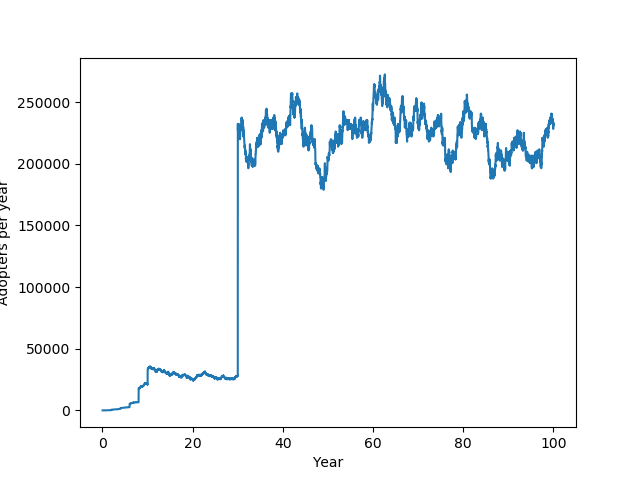
\includegraphics[width=0.5\textwidth]{adopter_per_year}
\caption{results}
\label{fig: adopters}
\end{figure}

\begin{figure}
\centering
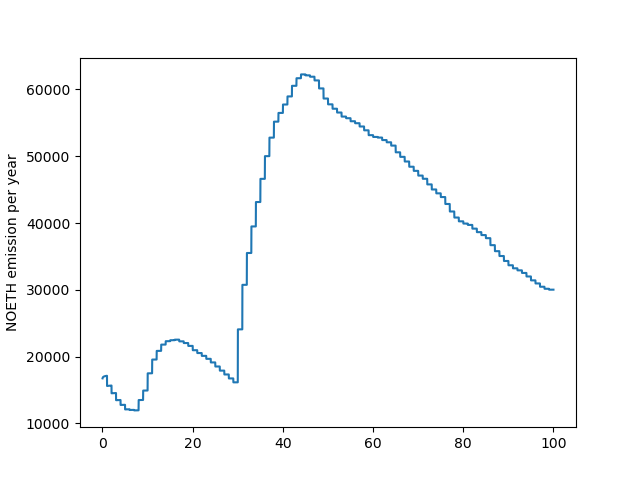
\includegraphics[width=0.5\textwidth]{noth_emission}
\caption{results}
\label{fig: noeth_emission}
\end{figure}

\begin{figure}
\centering
\includegraphics[width=0.5\textwidth]{total_circualtion}
\caption{results}
\label{fig: total_circulation}
\end{figure}

\section{A credit system for measuring computing power}\label{sec:credit-system}
\section*{How to spend the token}


\begin{thebibliography}{MPP}
	\bibitem[KM]{kermack} Kermack William Ogilvy and McKendrick A. G. \emph{A contribution to the mathematical theory of epidemics}. Proc. R. Soc. Lond. (1927) A115700-721.
	\bibitem[PS]{peruanisibona} Peruani, F. and Sibona, G.  \emph{Reaction processes among self-propelled particles}. Soft Matter (2019), vol. 15, 497.
	\bibitem[V]{verhulst} Verhulst, P.-F.\emph{Recherches math\'ematiques sur la loi d'accroissement de la population}. Nouv. M\'em. Acad. R. Sci. B.-lett. Brux. 18, 1-45 (1845).
\end{thebibliography}
\end{document}